
%
%  $Description: Author guidelines and sample document in LaTeX 2.09$
%
%  $Author: ienne $
%  $Date: 1995/09/15 15:20:59 $
%  $Revision: 1.4 $
%

\documentclass[10pt,twocolumn,ieeetran]{article}
\usepackage{latex8}



\usepackage{picture}
\usepackage{listings}
\usepackage{tikz}
\usepackage{verbatim}
\usepackage{pgf-pie}
\usetikzlibrary{shapes,decorations}
\usetikzlibrary{decorations.text}
%\usepackage{marvosym}
\usepackage{amssymb}
\usepackage{fancyheadings}

\usepackage{pgfplots}
%\usetikzlibrary{chain}

\usetikzlibrary{shapes.callouts}
\usepackage{theorem}
\usetikzlibrary{decorations.pathmorphing,backgrounds,fit}

\usetikzlibrary{arrows,shapes.misc,chains,positioning,scopes,calc,through,backgrounds,fadings} 

\usetikzlibrary{mindmap,trees}

\usepackage{pgfplots}
\usetikzlibrary{patterns}
\usetikzlibrary{calc,3d}


\usetikzlibrary{shapes,snakes}
\usepgflibrary{decorations.markings}

%\documentclass{book}

\usetikzlibrary{calendar} % LATEX and plain TEX

%\usepackage{times}

%\documentstyle[times,art10,twocolumn,latex8]{article}
\usepackage{tikz}

%-------------------------------------------------------------------------
% take the % away on next line to produce the final camera-ready version
\pagestyle{empty}

\usepackage{tikz}

\tikzset{ 
  nonterminal/.style={ 
    % The shape: 
    rectangle, 
    % The size: 
    minimum size=6mm, 
    % The border: 
    very thick,           
    draw=red!50!black!50, % 50% red and 50% black, % and that mixed with 50% white 
    % The filling: 
    top color=white,               % a shading that is white at the top... 
    bottom color=red!50!black!20, % and something else at the bottom 
    % Font 
    font=\itshape                 
  }, 
  terminal/.style={ 
    % The shape: 
    rounded rectangle, 
    minimum size=6mm, 
    % The rest 
    very thick,draw=black!50, 
    top color=white,bottom color=black!20, 
    font=\ttfamily}, 
  skip loop/.style={to path={-- ++(0,#1) -| (\tikztotarget)}} 
} 

\newcommand{\marginlabel}[1]{\mbox{}\marginpar{\raggedleft\hspace{0pt}#1}}
\tikzstyle{every node}=[font=\small, text centered, node distance=1.5cm] 
\tikzstyle{decision} = [diamond, draw, fill=red!20, 
    text width=4.5em, text badly centered, node distance=2cm,minimum height=0.6em, inner sep=0pt]
\tikzstyle{block} = [rectangle, draw, fill=blue!20, 
    text width=7em, text centered, rounded corners,  minimum height=0.5em]
\tikzstyle{line} = [draw, -latex']
\tikzstyle{cloud} = [draw, ellipse,fill=red!20, node distance=3cm,
    minimum height=2em]

\newenvironment{matrixtable}[4]{%
  \begin{tikzpicture}[matrix of nodes/.style={
    execute at begin cell=\node\bgroup\strut,
    execute at end cell=\egroup;}]
  \matrix (m) [matrix of nodes,top color=violet!40,
    bottom color=violet!80,draw=white,
    nodes={draw,top color=violet!35,bottom color=violet!45,
    draw,inner sep=2pt,minimum height=3.1ex},
    column sep=0.2ex,row sep=0.2ex,inner sep=0.5ex,
    rounded corners,column 1/.style={minimum width=#1},
    column 2/.style={minimum width=#2},
    column 3/.style={minimum width=#3},
    column 4/.style={minimum width=#4}]}%
{;\end{tikzpicture}}

\tikzset{ 
  nonterminal/.style={ 
    % The shape: 
    rectangle, 
    % The size: 
    minimum size=6mm, 
    % The border: 
    very thick,           
    draw=red!50!black!50, % 50% red and 50% black, % and that mixed with 50% white 
    % The filling: 
    top color=white,               % a shading that is white at the top... 
    bottom color=red!50!black!20, % and something else at the bottom 
    % Font 
    font=\itshape                 
  }, 
  nontermina2/.style={ 
    % The shape: 
    rectangle, 
    % The size: 
    minimum size=6mm, 
    % The border: 
    dotted,           
    draw=red!50!black!50, % 50% red and 50% black, % and that mixed with 50% white 
    % The filling: 
    top color=red,               % a shading that is white at the top... 
    bottom color=red!50!black!20, % and something else at the bottom 
    % Font 
    font=\itshape                 
  }, 
  terminal/.style={ 
    % The shape: 
    rounded rectangle, 
    minimum size=6mm, 
    % The rest 
    very thick,draw=black!50, 
    top color=white,bottom color=black!20, 
    font=\ttfamily}, 
  skip loop/.style={to path={-- ++(0,#1) -| (\tikztotarget)}} 
} 

%-------------------------------------------------------------------------

%%%%%%%%%%%%%%%%%%%%%%%%%%%%%%%%%%%%%%%%%%%%%%%%%%%%%%%%%%%%%%%%%%
% PARA ELIMINAR TODAS LAS NOTAS DE UNA VEZ DESCOMENTAR LA DEF VACIA
%%%%%%%%%%%%%%%%%%%%%%%%%%%%%%%%%%%%%%%%%%%%%%%%%%%%%%%%%%%%%%%%%%
\usepackage{xcolor}
%\newcommand{\revisar}[1]{{\color{red}[#1]}}
\newcommand{\nota}[1]{{\color{red}[#1]}}
\newcommand{\revisar}[1]{}
%\newcommand{\nota}[1]{}
\newcommand{\nonota}[1]{#1}

%-------------------------------------------------------------------------


\title{Towards a Social Interaction-based Cognition Model: An Analysis of Spatial Data Infrastructure}

\author{Luis Reynoso, Eduardo Grosclaude, Laura S\' anchez \\
Facultad de Inform\' atica\\ {\it Universidad del Comahue, Argentina} \\
{\it Buenos Aires 1400 (8300) Neuqu\'en}\\ \{Luis.Reynoso, Eduardo.Grosclaude,  Laura.Sanchez\}@fai.uncoma.edu.ar\\
% For a paper whose authors are all at the same institution,
% omit the following lines up until the closing ``}''.
% Additional authors and addresses can be added with ``\and'',
% just like the second author.
\and
Mabel \' Alvarez\\
{\it Universidad de la Patagonia San Juan Bosco, Argentina}\\
{\it Belgrano y Rawson (9100) Trelew, Chubut}\\
mablop@speedy.com.ar\\
}


% Java Code: 
\lstdefinelanguage{Java}{morekeywords={print,while,def,for,in,range,public,double,static,void,class,method,int,if,else,new,main,boolean,type,strings,char,package,private,null},
keywordstyle=\color{blue}\bfseries\sf,sensitive=false,morecomment=[l]{//},morecomment=[s]{/*}{*/},morestring=[b]",}
\lstset{language=Java, basicstyle=\normalsize, numbers=none, numberstyle=\bf, tabsize=2}
\definecolor{gg}{rgb}{0,90,0} % definicion rgb para un color
\definecolor{comentarios}{rgb}{150,150,150} 
\lstset{morecomment=[l][\color{gray}\bfseries\sf]{//}}
\lstset{stringstyle=\color{orange}\bfseries\sf}
\lstset{morestring=[b][\color{orange}\bfseries\sf]{"}{"}
}
% fin Java Code


\begin{document}
\maketitle
\thispagestyle{empty}




\begin{abstract}
Distributed cognition is a psychological theory which assumes that knowledge lies not only within the individual but also in the individual's social and physical environment. Today, we tend to achieve cognitive results by means of a sequence of complex and subtly interwoven interactions, using  technological devices, and with the help of other, more knowledgeable people. As dwellers of a new century, we are agents of a novel technological assembly where knowledge is socially produced, and nurtured by the various sources of many communities of practice (CoP). In this paper we propose a social interaction-based cognition model which applies distributed cognition and interoperability between different actors of CoP in a web environment. The core components of the model are Authenticity and Cohesion, Assemblage and Shared Meanings. We also present the main findings of qualitative research in a case of study to Spatial Data Infraestructure (SDI) and CoP around this technological assemblies. 
%Requeriments to built an SDI includes: to share a common representation of the space according to different aspects: administrative, technical, semantic interoperability, to work in CP and to apply distributed cognitions and conceptions. 
% the social coordinations about their space
% http://tecfa.unige.ch/tecfa/publicat/dil-papers-2/

\end{abstract}

{\bf Keywords:} Social Interaction. Distributed Cognition. Communities of Practice. Interoperability. 


%-------------------------------------------------------------------------
\Section{INTRODUCTION}


%Cognitive theories show a strong vias toward an analysis of the individual while thinking and learning.
Studies have traditionally considered cognitive processes \cite {Wang2005} and development as something possessed by individuals and residing in their heads. Accordingly, cognitive models have been reduced to the process being carried out by an individual.  
However, thinking and learning often involve giving up some higher-order knowledge and executive functions to the environment in worthwhile ways. 
From a distributed-cognition-based perspective, 
the person and its surround are taken into account as a single system 
in order to analyze  thinking and learning contexts and processes. 
As for the person's surround, both social and technological factors need to be considered. Both undoubtedly contribute to cognitive development; they are more than external sources of stimulation.

The social development theory by Vygotsky \cite{Wertsch} constitutes an important framework 
dealing with the social surround of the learning process. Vygotsky's theory involves an individual, with the help of {\it more knowledgeable others} ({\it MKO} in Vygotsky's theory), in a {\it zone of proximal development (ZDP)} environment. Our reasoning can be expressed in this way: without help from others, much of our ablest learning, such as that resulting from interaction between the individual and {\it MKO},  could not be performed. Distributed cognition describes the cognitive aspects which are triggered between these individuals involved in the process, with the consideration of technological resources and environment.

The theory of distributed cognition \cite{Salomon} does not oppose to existing cognitive theories of the isolated individual. It rather encompasses those theories within a wider model where cognitive aspects are not just produced by an individual but also by the interaction among subjects, and between subjects and their environment.

We believe that the topic of interaction is what remains to be studied in existing cognitive models. The study of social interaction and cognitive interaction will contribute to understand social cognition and build knowledge of humanity \cite{Denny} that endures and keeps growing on beyond the lives of individuals.

In such a study, the application of distributed cognition could be \nonota{complemented with theories of } communities of practice ({\it CoP}) \cite{Wenger} and social networks ({\it SN}) \cite{Kadushin}\cite{Santos}\cite{Watts}. When we work in a social network, as well as in CoP, we need to think of ourselves as an interwoven chain of nodes that interacts between each other. A social network is a social structure made up of social actors (nodes), such as individuals, groups or organizations \cite{Wasserman}\cite{Jamali}. CoP are present in organizations as much as in our ordinary life, as they are a facet of social networks.

%  such as  IDERA in Argentina, INDE in Brasil, IDEE in Spain, European SDI INSPIRE, etc.
We focus on interoperability of actors within social and technological environmental interactions, as well as on analyzing which roles are performed by actors in these contexts. We show findings obtained from qualitative 
research we performed with communities of practice belonging to Spatial Data Infrastructures ({\it SDI}). 

SDI emerged as a technological solution of this century to manage and analyze physical space (land and water). 
Technological assemblies of organizations within a SDI have evolved and improved in several countries, at different scales (local, national, regional). SDI requires that each organization participating in building the data infrastructure contributes by providing its own space information (or spatial ability) within a common information framework. Spatial information is shared by means of common technology to allow the space to be visualized, analyzed and managed accordingly. To build such an infrastructure (SDI), social, cultural \cite{Nisbett} and cognitive changes should take place within intertwined communities.

%To address a study of distributed cognition will give us more elements to understand the collective knowledge that remains in the time between communities, regions and the global society. Knowledge that remains through the interaction of oral society, after the legal society and this time with other technological items.


           
The paper is organized as follows. Section 2 introduces the theory of Distributed Cognition. 
Section 3 provides an overview of Communities of Practice. Section 4 describes Interoperability. Section 5 presents a Y-model of the Social Interaction-based Cognition. 
Section 6 details a case study of Communities of Practice and interoperability of SDI. 
Section 7 goes on to describe conclusions and future work.
                                       
                                                     
\Section{DISTRIBUTED COGNITION}

This theory was originally developed in the mid-1980s by Edwin Hutchins. Using insights from sociology, cognitive science, and Vygotsky's psychology  (cf. cultural-historical psychology), it emphasizes the social aspects of cognition. The theory provides a balanced theoretical treatment of problem solving in real work situations, and supplies a new framework for cognitive science in general.
Distributed cognition has been proposed as a new foundation for human-computer interaction \cite{Hollan}. 

Distributed Cognition diverges from previous cognition theories in that it employs a variable unit of analysis.  Traditional cognitive theory takes the individual person as the proper unit of analysis.  In this traditional view, cognitive processes are internal processes.  Social, technological and cultural context is thus often left out of the analysis. In contrast, the theory of distributed cognition makes a larger cognitive system out of the individual and its socio-cultural context, one that is to be analyzed in a broadly traditional way, such as a computational system. 
Enlarging the unit of analysis in this way has the advantage that representations internal to the system are now external representations with respect to the individual agents that use and make use of them. 
So, distributed cognition is conceived as a system that entails both person and surround \cite{Salomon}.

Distributed Cognition can be considered as aligned with: (1) Vygotsky, whose cultural-historical theory \cite{Wertsch} locates individual cognitions within, rather than just interacting with, social and cultural contexts of interaction and activities \cite{Salomon}; and (2) Cole, who had pointed out \cite{Cole} that the proper unit of psychological analysis should be the joint socially mediated activity in a cultural context.

%The first and most fundamental rule according Durkheim \cite{Durkheim} is: Consider social facts as things.
%sociology of the technology \cite{Thomas}

Perkins \cite{Perkins}\cite{Perkins2} introduces a learning model within Distributed Cognition in which he proposes not to take as the unit of analysis the learner detached from the resources in his or her surround --the {\it person-solo}, but the {\it person-plus surround}, or person-plus for short. People employ the surround to support, share and undertake outright aspects of cognitive processing. Such is the perspective taken by the person-plus on thinking and learning contexts, to treat the person plus surround as one system.
He also introduces the concept of {\it equivalent access hypothesis}, which distinguishes four factors: the kind of knowledge, the way it is represented, how readily it is retrieved, and how it is constructed \cite{Salomon}.

Existing literature includes many examples of distributed cognition. They are diverse with varying complexity. Simple examples involve problem-solving using pencil and paper or computers, to more complex metaphors in the context of navigating a navy vessel, or crewing a plane \cite{Hutchins95}. 
%counting as part of the thinking what gets done or partly done in the surround (perkins)


We think that the study of distributed cognition may alleviate cognitive drawbacks of learning designs based on traditional cognitive models: 

\begin{itemize}

\item People often fail to apply knowledge and skills learned in one context to other situations \cite{Perkins} (cognitive transfer). Distributed cognition emphasizes collaborative learning, learning by practice and learning within communities of practice.

\item People often fail to decontextualize\footnote{Decontextualizing \cite{Wertsch} is the handling of information in a way that either disconnects other information or backgrounds it \cite{Denny}. It is produced when the meaning of  signs is becoming less dependent on the spatial and temporal context in which they are used. For example, when we induce a general rule for a set of observed facts, we abstract/produce a common structure behind the observed cases, so shifting of propositional levels occurs.}: Cognitive decontextualization is a required cognitive activity prior to applying cognitive transfer.  

\item People often fail to solve problems applying mediator instruments (such as technological resources).
Cognitive distribution considers that thinking and learning often involve relinquishing some higher and executive function to the surround in worthwhile ways. Usually, this relinquishing includes the use of technological devices and resources which should be taken into account. Distributed cognition analyzes the interaction between subject and objects.   
\end{itemize}



%Social Networks \cite{Santos}, \cite{Watts}.





\Section{COMMUNITIES OF PRACTICE}

Learning is not an activity that can be carried out in isolation. We learn from other people, either from the culturally produced artifacts that provide mediator elements \cite{Wells}. Wells \cite{Wells}  argues that to understand learning we need to understand how an individual, as a member of a community, applies and produces representations in the collaborative effort to transform their shared world.

% conocer no es una actividad que se pueda llevar a cabo en aislamiento, aprendemos bien de otras personas o bien de los artefactos culturalmente producidos que proporcionan los elementos mediadores. (Wells 2001)

%as pointed out by Cole \cite{Salomon}

Wenger \cite{Wenger} argues that the primary unit of analysis (in sociological studies) is neither the individual nor social institutions but rather the informal communities of practice that people form as they pursue shared endeavors over time \cite{Wenger}. The author emphasizes that engagement in social practice is the fundamental process by which we learn and so become who we are. Three processes for individual and group identity formation are identified in communities of practice, as the key elements for individual membership identity as well as for developing community identity: (1) mutual engagement, (2) joint enterprise, and
(3) shared repertoire.


Learning takes place during active participation in a social group, which not only allows the individual to become a member, but also provides the elements for that individual to construct an identity through these communities. Individual identity, as well as social identity, affects the perception of the group and its common repertoire. Perception, in consequence, affects cognition and influences  its tasks.

%Las comunidades de practicas estan compuestas por actores que pueden ser organismos.-
\Section{INTEROPERABILITY}

%A property of distributed cognition is its constituents be interchangable. 
When analyzing distributed
cognition in web environment, access to resources and interactions between actors is key. Distributed cognition
is not conceived without communication, or without ability of its members to communicate.

Interoperability is the ability of making systems and organizations to work together (inter-operate). People (or organizations) working within an interoperability environment should develop a capacity or ability to exchange (and retrieve) knowledge, as well as to use the exchanged knowledge and to build new one upon them. 
While the term {\it interoperability} was initially defined for information technology or systems engineering services  allowing for information exchange, a broader definition takes into account social, political, and organizational factors that impact system-to-system performance.

The three dimensions of interoperability include:

\begin{itemize}

\item Technical interoperability: pertains to the technical issues required to ensure that the technological components of the participating actors' information systems  are prepared to work together. Therefore  it allows to provide common mechanisms for transferring data and invocation of functions, transparent to networks substratum and information systems (applicable to multi-platform, multi-language systems). Interfaces, interconnection services, data integration, middleware, data presentation and exchange, accessibility, open systems and secure systems, among other items,   pertain to technical interoperability. It involves the use of technology to manage information structure, the structure of services, semantics of information, and semantics of web services \cite{Moreno}. The technical dimension of interoperability allows us to analyze an economic perspective of  interoperation between actors. When considering the different roles that the actors can take in terms of consumer/producer, or supply/demand information (or even other roles from the ISO Model for Open Distributed Processing, {\it RM-ODP}) we can have a clear view of  information flow and traffic.

\item Semantic interoperability: It deals with meaning in the use of data and information and, in particular, ensures that the precise meaning of exchanged information can be understood by any application. The information must be interpreted in an univocal manner. Actors usually handle their own definitions of information, which often introduces a disadvantage for the exchange of information. The information that is unequivocally performed is easier to be exchanged and interpreted, ensuring an adequate flow of information \cite{Moreno}.
In this matter it is necessary to comply with a formal mechanism to define common elements. This mechanism should ensure quality, and must be accepted and respected. Formal documentation that defines the data  must  be formally managed, allowing  the actors to maintain reliability.  On the other hand, they should be disseminated by the mass media, being  available to every actor. Additionally, if the definitions are adapted to new requirements,  backward compatibility  with previous definitions   must be  guaranteed. Some of the tools available are classification systems, thesaurus, metadata, and ontologies. 

\item Organizational interoperability: This deals with the definition of: (1) business goals, (2) modeling business processes, and (3) facilitates the collaboration of administrations that wish to exchange information by maintaining different structures and internal business processes of government \cite{Moreno}.

Organizational interoperability ensures alignment of administrative procedures involved in the provision of e-government services. In practice this means  defining, collaboratively, the why and when  of  the trading of information, rules and regulations that ensure safety in such trade or plans that will guide the implementation of the initiatives.
It is also responsible for analyzing the gaps in provision of information and even  responsibility overlaps in information and processes \cite{Moreno}. In other words,  it attends  the analysis of boundaries, scope and information links and processes between actors.
\end{itemize}


The semantic dimension of information exchanged and its own interpretation is related to the perspective of the symbolic space of society. For example, an ontology is the conceptualization of collective concepts and semantic relationships established between them in a particular domain.
This collective conceptualization is itself a symbolic construction which in turn is based on cognitive and individual representations of the domain. Finally, it is important to note that in the field of symbolic space also resides the public sphere and field of action of civil society, and it is from these that modifications to the new social space are made.
It is through the symbolic space that individuals and institutions can demonstrate their agency capacity  \cite{Bandura}. This is often an individual agency capacity, but in an interoperable space  it can be developed as a whole, and affects their immediate environment ({\it proxy agency} in the theory of Bandura \cite{Bandura}).


The organizational dimension of interoperability is related to Castells's administrative perspective in \cite{Castells2}. The determination of business processes and competencies of the interoperating social partners must be analyzed using a formal, legal framework. This framework must  allow to formalize what is exchanged, when information is exchanged and what means of security are implemented. These formal frameworks are part of the rules of the institutions. In terms of social capital, a concept corresponding to the networks and norms that facilitate collective action \cite{Woolcock} \cite{Uphoff} \cite{Dahal} \cite{Sobel} \cite{Maseda}. Administrative interoperability is rather related  to the rules associated with the social capital of a society, while networks concern to its technical dimension. Determination of gaps or overlap in information will affect new legislation, which facilitates the adoption of new regulations on the subject.


\subsection{Technical Interoperability}
In this section technical interoperability is described in more detail. Technical interoperability describes the system in terms of economic aspects of the relations of production/consumption, supply/demand and the technology used. The RM-ODP model can be applied and used in the study of these forces of production considered in this aspect of interoperability. A distributed model is useful to describe a system regarding data and services provided by stakeholders, whose functions are producers and consumers of data-services, thus contributing to a richer view of the system.

Stakeholders can be categorized according to their roles, which will be briefly described below (refer to Fig. 2 for short identification tags).

Producer (PRD): An actor who produces data or services. Provider (PRV): An actor who provides data or services to users. The provider differs from the producer, because an actor can serve as support in providing service without having produced the original data. Political decision maker (Policy Maker, PM): An actor that sets economic policies implemented (or needed) by a group of those involved. Broker (BRK): An actor who provides assistance to users and providers and assists in negotiating contracts between them and can maintain metadata records on behalf of an owner of a product. Their functions include metadata gathering of producers and suppliers, creating catalogs and providing services based on these catalogs. Value Added Reseller (VAR): An actor that adds some feature to an existing product or group of products, and then makes it available as a new product. End User (EU): An actor who uses the information for a specific purpose; an actor with legitimate interest in the use and consumption of data or services provided by other actors.


\Section{SOCIAL INTERACTION-BASED COGNITON}

Computer science has never been alien to the human component within which it is developed, for example by addressing the study of human-computer interfaces, the elicitation of system requirements, etc. In particular, software engineering itself is an inherently human discipline and its measurement makes it closer to the social sciences than the physical sciences \cite{Morasca},  because the phenomena addressed rely on human behavior and these are not easily controlled.
During the last decades,  many human factors and learning characteristics of those who interact with software have been taken into account (for instance, the study of human-computer interface, the study of the correlation between learning styles of users and specific software, etc.) as well as transcultural and global factors in their development (e.g. global software engineering).
Likewise, when the government's task calls for reaching  out to citizens through transparent and accessible mechanisms in e-government,  the efforts in the study of government policies have been moving closer to the social sciences, \cite{Graham}. E-government applications aimed at providing citizens with single-window functionality bring a unique view, detached from any internal partition into separate units that the government might  have \cite{OECD}.
However, the advent of the Internet and the adoption of social networks have given a new significance to  opinion formation and communication in society as an important object of study that serves as input for decision-making by governments and market policies.
We should highlight in this type of study the areas of growing importance that are no longer in the individual or institutional spectrum but in the social approach, e.g. Studies on Collective Intelligence \cite{Seragan}, Social Web Applications \cite{Bell}, Social Network Analysis \cite{Tsvetovat} and Computational Sociology. These technologies, applied to the design and analysis of social networks, may allow a better approach to civil society and the public sphere (e.g. they have been used in political campaigns with a strong presence in social networks). Thus, we can argue that the social field is an increasingly significant one.

\subsection{THE PROPOSED Y-MODEL}

The Social Interaction-based Cognition ({\it SIbC}) has three dimensions: CoP, CD and Interoperability. Each one of them presents three components as shown in  Fig. 1  through a Y-model. It is named a Y-model simply because SIbC dimensions  are shown over a Y-shaped diagram. The dimension components complement each other, as they are semantically connected.

The outside circle of the Y-model shows the cohesion of Social interaction, which is primarily based of technical interoperability abilities in establishing (dyadic, triadic, etc.) ties between actors through social nets, in maintaining strong and weak interactions. The actors (individual or organizations) of those social interactions reveal specific roles (authenticity).

\begin{figure}[htpb,scale=0.3]
  \centering
  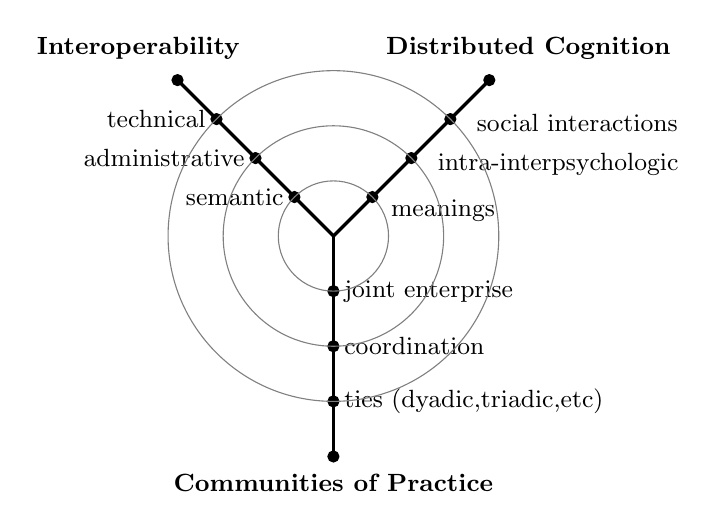
\begin{tikzpicture}[>=stealth',line join=bevel,font=\sffamily,auto,on grid,decoration={markings,mark=at position .5 with \arrow{>}}] 
    %\input{y_chart_common}
    \coordinate (behaviouralNode) at (135:3.5cm);
    \coordinate (structuralNode) at (45:3.5cm);
    \coordinate (physicalNode) at (270:3.5cm);
    \coordinate (originNode) at (0:0cm);

    \node [above=-1.0em] at (behaviouralNode) {\textbf{Interoperability}};
    \node [above=-1.0em] at (structuralNode) {\textbf{Distributed Cognition}};
    \node [below=-1.7em] at (physicalNode) {\textbf{Communities of Practice}};

    \draw[-, very thick] (135:2.8cm) -- (0,0) node[left,pos=0.25]{technical} node[left,pos=0.5]{administrative} node[left,pos=0.75]{semantic};

    \draw[-, very thick] (45:2.8cm) -- (0,0) node[pos=0.15]{social interactions} node[pos=0.4]{intra-interpsychologic} node[pos=0.7]{meanings};

    \draw[-, very thick] (270:2.8cm) -- (0,0) node[right,pos=0.25]{ties (dyadic,triadic,etc)} node[right,pos=0.5]{coordination} node[right,pos=0.75]{joint enterprise};

    \draw[fill] (barycentric cs:behaviouralNode=0.8,originNode=0.2) circle (2pt);
    \draw[fill] (barycentric cs:behaviouralNode=0.6,originNode=0.4) circle (2pt);
    \draw[fill] (barycentric cs:behaviouralNode=0.4,originNode=0.6) circle (2pt);
    \draw[fill] (barycentric cs:behaviouralNode=0.2,originNode=0.8) circle (2pt);

    \draw[fill] (barycentric cs:structuralNode=0.8,originNode=0.2) circle (2pt);
    \draw[fill] (barycentric cs:structuralNode=0.6,originNode=0.4) circle (2pt);
    \draw[fill] (barycentric cs:structuralNode=0.4,originNode=0.6) circle (2pt);
    \draw[fill] (barycentric cs:structuralNode=0.2,originNode=0.8) circle (2pt);

    \draw[fill] (barycentric cs:physicalNode=0.8,originNode=0.2) circle (2pt);
    \draw[fill] (barycentric cs:physicalNode=0.6,originNode=0.4) circle (2pt);
    \draw[fill] (barycentric cs:physicalNode=0.4,originNode=0.6) circle (2pt);
    \draw[fill] (barycentric cs:physicalNode=0.2,originNode=0.8) circle (2pt);

 %   \draw[black!50] (0,0) circle (4.0cm);
 %   \draw[black!50] (0,0) circle (3.2cm);
    \draw[black!50] (0,0) circle (2.1cm);
    \draw[black!50] (0,0) circle (1.4cm);
    \draw[black!50] (0,0) circle (0.7cm);

  \end{tikzpicture}
  \caption{Y-Model of Int-based Social Cognition} 
  \label{figure:gajski_kuhn_y_chart__levels_of_abstraction}
\end{figure}


The middle circle of the Y-model accounts for the claim that social interactions are based in confidence and assemblage links. Assemblage is the product of dialectic processes that reside within the intra and inter-psychological plane \cite{Wertsch} producing internalization and externalization of actions. Assemblage in social interactions manifests as summary communication between actors when they are conscious in collaboration tasks avoiding overlapping, or when the 'shared experience' shrinks communication or action. This property is materialized between actors through abstract informal links like confidence, or through objective formal relationships of social contracts (or social procedures).

The inside circle of the Y-model displays the inner core of the model: a joint enterprise is a social construction based in shared meanings between actors, implying a semantic interoperation around a joint repertoire. 


%. Requirement n 1- Commitment The participants recognize the benefits and value of the relationship and are determined to make it work. The level of commitment should progress with time, and the level of responsibility and interaction should increase as the relationship develops. 

%Requirement n 2 - Authenticity Relationships require honesty and candor on both sides. It would be notice if the expressions of care are not sincere, and the relationship will go backwards On the other hand, genuilly expressed appreciation will be quickly perceived and accelerate the evolving relationship. 

%Requirement n 3 - Communication Both parties should feel free to express themselves as they are and known that they will be heard and understood. 

%Governance studies all mechanisms, processes and rules through which ,  economic, political and administrative authority   in an organization, both business and government or the third sector (NGOs) is exerted.  It is a concept that aims to describe a complex systemic transformation that occurs at various levels, from local to global, and among different stakeholders in the public, private and civil sectors. Addressing this concept means tackling social and spatial problems. Social, because it is fundamental both the search for balance and stability of the actors in government of the public and private spheres, as the study of their opinion, perception and participation on the policies and actions of government; and also spatial because it is important to consider the space of configurations adopted by these actors and the adequate management of their own space and resources.  In terms of analyzing each actor we must  pay attention to  which their capacity  / ability is to exchange information and to use the exchanged information, it means, we must consider their level of interoperability.


%social formations are assemblages of other complex configurations, and they in turn play roles in other, more extended configurations.


% !! capacidad de agencia proxy??



\Section{A CASE STUDY: SDI}
In this century, land management's organizations have tended to use Spatial Data Infrastructure (SDI) technologies to interoperate with  society. SDI allows a shared infrastructure which integrates each data source to co-produce the same space. Spatial information with the help of SDI is the result of the integration of different geographical objects which are produced and maintained by each land manager.

Spatial Data Infrastructure have been adopted by many land management communities around the world such as   INDE in Brasil, IDEE in Spain, European SDI INSPIRE, etc., and their associated technologies are widespread. However, land management organizations have undergone a profound shift from the original use of GIS (in isolation) towards the participation within SDI.
This change was cultural, cognitive and organizational.

We adopt a qualitative and inductive methodology running several unstructured interviews in Neuqu\' en province and others communities of Argentina implementing SDI. We study the interactions of several actors within SDI, we focus on their roles, their interoperabilities, cognitive changes and demands, and the benefits of working in communities of practice.  Interviews help us to identify and characterize role
categories of SDI actors.


Noucher \cite{Noucher1} also applies qualitative research in the study of appropriation stages of spatial datasets; however she takes a Piagetian approximation (identifying assimilation and accomodating stages). 
Our Vygotskian approach is not separated from the social context; we do not study stages, but roles of SDI actors which are inherent to the goals of their organization. We also study their interaction through interoperability and CoP.

%! when sdi actors help other as they participates, communication with peers and scaffolding take place

In this section we describe the main findings of our case study. The section is divided as follows. The first section describes SDI and communities of practice. The following details the interoperability around SDI. In the last section, cognitive aspects around SDI are included.
 
%Early work in distributed cognition was motivated by the basic insight that cognition is a socially (also, materially and temporally) distributed phenomenon, one that is essentially situated in real practices (Hutchins 1995a).  The theory does not posit some new kind of cognitive process.  Rather, it represents the claim that cognitive processes generally are best understood as situated in and distributed across concrete socio-technical contexts. 

\subsection{CoP AROUND SDI}


SDI communities of practice are not only a way of sharing knowledge and know-how of stakeholders about land management. They are important mediator instruments to hold the agreement of the collective negotiation which allowed  the SDI to be defined. However, these SDI actors need to work with spatial data which is the result of collective negotiation as well as the object of individual representation \cite{Noucher1}. Technologies to manage internal geographical data (of the organization) are not exactly the same as those applied to interoperate in SDI, neither in their cognitive representation, nor in the interpretation applied. However, a set of patterns can be identified in geographical management and analysis. Common experience in dealing with its problem-resolution can be exchanged, giving a suitable context to articulate communities of practice.  

In the last two years, a regional broker (OPTIC) of the province of Neuqu\' en (Argentina), has been trying to foster the sense of belonging in different organizations to communities of practice around SDI.
OPTIC asked for the designation of organizations' leaders to participate in land management communities. The SDI communities of practice are: Legal, Data Market, and Geographical Data. This province's SDI is being built up from the work of these leaders working in communities of practice.

\begin{itemize}
\item The Data Market Community allows the SDI stakeholders to analyze their data in terms of a data system of offer and demands. Each organization must provide a particular set of data and is granted access to a set of data provided by others it's interacting with. In this community, the leaders are motivated to verbalize related problems and to reason applying their organization's point of view to the interactions. This community is the source for defining and maintaining web services of geographical data.
 
\item Legal Community allows the SDI stakeholders to concentrate in legal aspects. SDI requires administrative interoperability to avoid overlapping of functions, to ensure the provision and consumption of data, to change the isolated methodologies of a standalone organization to those of one emphasizing source of information; etc.
\item Geographical Data  community is intended to support the organizational internal work of each stakeholder in producing and managing its data. The community promotes the sharing of know-how in using GIS technology according to their internal goals within the framework of SDI policies.
\end{itemize}

Noucher et al. \cite{Noucher2} reported other SDI communities of practice in France, Canada and Switzerland.
The authors \cite{Noucher1} argue that a community of practice, viewed as a learning network, offers one of the most important component examples of territorial intelligence.

\subsection{INTEROPERABILITY IN SDI}

The SDI represents infrastructures that allow the exchange and interoperability of geographic information among multiple stakeholders (public sector, private, academic, non-governmental and civil society). During the last decades the exchange of geographic information was digitally systematized by multiple organizations in different contexts in order to serve different purposes \cite{Delgado} \cite{Georgiadou}.
Initially the exchange of geographic information from different Geographic Information Systems (GIS) was performed by replicating data and converting data from one encoding mechanism to another, but this is a cumbersome practice whereby exchanges of information were scarce. The specification and adoption of international standards has allowed systems to interoperate with geographic information through SDI.
Web services applied to SDI allows to build the infrastructure consuming and providing data and services from different sources.


\subsubsection{TECHNICAL INTEROP.}

There are about 100 standards that can be considered as part of a software architecture of an SDI, and implementation of an interoperable geospatial solution \cite{Masser}.
The community of the Association for Global Spatial Data Infrastructure recommends adopting the definition of a relatively small set of standards (eg. WMS, WFS, etc.) as well as maintaining suitable metadata.

To illustrate the different roles of actors in a SDI we will mention one of each type for a SDI provincial scale in the province of Neuqu\' en in Argentina (see Fig. 2). Examples of information producers are the Registry of Property (RPI), the Provincial Directorate of Cadastre and Land Information (DPCeIT) and the Provincial Directorate of Revenue (DPR).
These three  mentioned actors  interoperate between them; the RPI sends updates of the legal ownership of land to the  DPCeIT; DPCeIT in turn sends economic information (tax valuations) and holders of formal and informal domain to the DPR. An example of a VAR actor in the province is the Provincial Bureau of Statistics which provides  aggregate statistical information from the information coming from other providers, as well as own sources.
The Secretariat for Public Management is considered a PM as it sets  the underlying policy of provincial SDI guidelines. The Provincial Office of Information Technologies (OPTIC) plays the role of broker, setting the negotiation between suppliers, producers, etc. Besides, OPTIC is also shown in Fig. 2 as a provider due to the fact that it provides Internet access to a producer. Currently the OPTIC Market is coordinating meetings regarding  data and services in order to orchestrate interoperation. The end users are taxpayers, citizens, property owners, etc.  within civil society.


%every node/.style={join}, every join/.style={-latex}
\begin{figure}[h]
\begin{center}
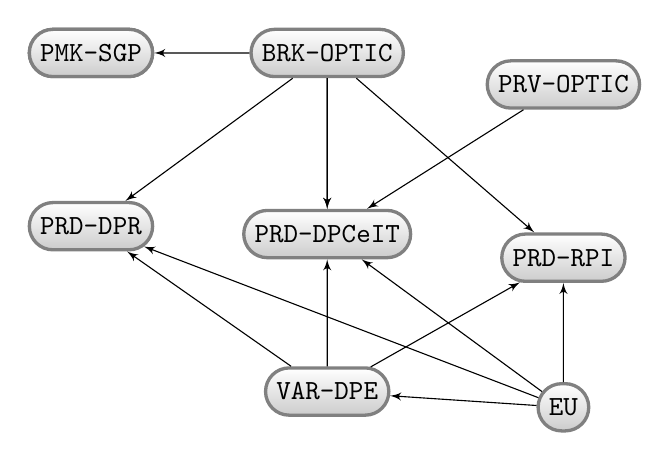
\begin{tikzpicture}[node distance=5mm]
\node [terminal] (sgp) {PMK-SGP};
\node [terminal, right of=sgp,xshift= 15mm, node distance=1.5cm] (optic) {BRK-OPTIC};
\node [terminal, right of=optic,xshift= 15mm, yshift= -4mm, node distance=1.5cm] (opticprv) {PRV-OPTIC};
\node [terminal, below of=sgp, yshift= -7mm, node distance=1.5cm] (dpr) {PRD-DPR};
\node [terminal, below of=optic, yshift= -8mm, node distance=1.5cm] (dpc) {PRD-DPCeIT};
\node [terminal, below of=opticprv, yshift= -7mm, node distance=1.5cm] (rpi) {PRD-RPI};
\node [terminal, below of=dpc, yshift= -5mm, node distance=1.5cm] (var) {VAR-DPE};
\node [terminal, below of=rpi, yshift= -4mm, node distance=1.5cm] (eu) {EU};
% Draw edges
\path [line] (optic) -- (sgp);
\path [line] (optic) -- (dpr);
\path [line] (optic) -- (dpc);
\path [line] (optic) -- (rpi);
\path [line] (opticprv) -- (dpc);
%% \path [line] (spg) -- (dpr);
%% \path [line] (spg) -- (rpi);
%% \path [line] (spg) -- (dpc);
%% \path [line] (spg) -- (var);
\path [line] (eu) -- (dpc);
\path [line] (eu) -- (dpr);
\path [line] (eu) -- (rpi);
\path [line] (eu) -- (var);
\path [line] (var) -- (dpc);
\path [line] (var) -- (dpr);
\path [line] (var) -- (rpi);
\path [line] (optic) -- (dpc);
\node [terminal] (sgp) {PMK-SGP};

   \end{tikzpicture}
\caption{Interactions between SDI Stakeholders}
\label{fig5}
\end{center}
\end{figure}


\subsubsection{ADMINISTRATIVE INTEROP.}
Perhaps the administrative interoperability, and even semantics, are the two areas in which progress has been lesser in terms of definition of SDI. The update of geographic data is a costly task. The SDIs facilitate the information to be provided and administered by the authentic sources of information, and  the geographic dataset from each source to be used and analyzed collaboratively. In this respect  the SDIs have facilitated the avoidance of costs  duplication  in time and effort, since it is not necessary  to duplicate  the information.
However, most SDI require more detailed analysis regarding the quality of the generated data, the overlapping  information when the competences of the sources are not clear, and the usage and interpretation of information. This topology of interoperability requires an exhaustive work,  a macro and collaborative analysis, as well as an agreement of the data flow and structure from larger scales.


\subsubsection{SEMANTIC INTEROP.}
While an SDI requires agreement on which technologies are applied in communication and collaborative work in relation to the management of one space, and an analysis of the associated business processes, an agreement is also needed about which data and metadata are exchanged. Delgado Fern\' andez et al. in \cite{Delgado} describe how the SDIs benefit from the common use of ontologies. 



\subsection{DC IN SDI}

Spatial data sharing and analysis require both a change on how SDI stakeholders think about themselves and how they think the space. With SDI, spatial knowledge is a consequence of a shared
co-production of the space by many actors (land management sectors such as planners, geologists, forester, etc.) so the stakeholders should not be working in isolation but within social networks. SDI introduces a change
in the identity of the organization. It does not change its organizational goals but modifies the way to obtain them through collaborative work with the help of more knowledgeable others.

Besides, SDI introduces epistemological, hermeneutical, cognitive and sociological issues. The fact that the knowledge of space is structured differently than when an organization works in isolation, introduces epistemological changes. The fact that SDI stakeholders should use a shared representation of the space knowledge implies to apply a shared interpretation (we need to study hermeneutic issues). Distributed cognition behind SDI involves also interpretation of spatial data which is the product of collective negotiation. 


Cognitive and sociological issues reinforce the sense of belonging to spatial communities \cite{Noucher2}, as well as facilitate and hinder, at the same time, the attribution of common meaning to data \cite{Noucher1}.
SDI unveils shared meaning \cite{Noucher1}, materializing the geographical interactions needed to work in collaboration, which are inherent of a common representation of the space. 
These new technological objects are a product of reification of the social interaction (according to Durkheim \cite{Durkheim}, we should consider social facts as things), but they need to be appropriately defined, due to the fact that they are a product of  knowledge engineering and sustained cognitive activities performed by several organizations. 

% So, they stress the importance of the contribution of knowdledge theories. 
During data appropriation process Noucher et al. \cite{Noucher1} identify two different dialectic process  performed by stakeholders of land management: Individual projection and collective negotiation.
The former is based on expectation and experience of the stakeholder. The latter is based on participation
and reification process. 


\Section{CONCLUSIONS}

Technologies are usually mediator instruments of society helping its members to interact and interchange in performing their goals. With the introduction of web technologies 2.0 and 3.0, applications are built  upon a network of cooperating data services; users contribute important value added of their own data to those provided by the application, and the emphasis of the application is focused on the coordination and interactions. 
When technology is used as an instrument by communities of practice, or even by a more wider set of organizations, harmonization and orchestration of services are required, and members' roles and interoperability should be analyzed. 
These technological changes, demand profound cultural investments in members and organizations due to the fact that data is a shared resource and object of interchange; relationships and interactions are materialized vehicles in social networks with specific roles. This flow and interaction should be analyzed from cognitive theories. The (time- and cost-wise) investment of efforts are profitable; the analysis of aspects of cognition in distributed communities of practice allow substantial improvements in how knowledge is perceived, retrieved, transfered and applied (cognitive improvements).

%%!!!!Inherently, there exists many social factors contributing to cognitive development. 

We believe that societies facing such crucial process changes undergo important cognitive changes: knowledge is organized in a different way (introducing epistemological changes), and by consequence, this impacts in the way the society interpret the information it should deal (hermeneutic aspects that should also be considered). Our reasoning is that: distributed cognition (which enhances the understanding of interactions between humans, machines and environments) within communities of practice around web applications provides a suitable context to analyze the aforementioned problematic. Based on a set of interviews and the experience related to our case of study, spatial data infrastructure, we understand cognitive issues inside these communities. Data harmonization and services orchestrations required by these changes, also contribute to their sense of identity and improve its capacity of agency proxy. Community interoperability (ability of making systems and organizations to work together) plays a central role in the process of 'making meaning',
being perception of process information (issue of cognition) influenced by sense and meaning. 

%Social interaction in the development of cognition (Vygotsky) plays an important role in the process of 'making meaning'.
%Distributed cognition illustrates the process of interaction between people and technologies in order to determine how to best represent, store and provide access to digital resources and other artifacts.

%What distinguishes distributed cognition ....from other approaches also concerns to the boundaries of the unit of analysis for cognition.

As a future work we intend to continue to deepen the qualitative analysis of cognitive aspects that occur in these types of technological assemblies in society, applying methodologies of grounded theory which can guide us in a theoretical sampling of data. We also plan to apply focus group techniques within communities of practice.

%\vspace{0.2cm}

\noindent {\bf ACKNOWLEDGMENTS}

\noindent This research is part of projects  PI997/12: 'Hacia el Fortalecimiento de la Sociedad en el Uso y Aplicaci\' on Geoespacial y las TICS' of Universidad Nacional de la Patagonia San Juan Bosco and 04/F003 'Modelos y Tecnolog\' {\i}as para Gobierno Electr\' onico' of Universidad Nacional del Comahue.

\bibliographystyle{ieeetr}
\bibliography{latex8}

\end{document}

